%%%%%%%%%%%%%%%%%%%%%%%%%%%%%%%%%%%%%%%%%%%%%%%%%%%%%%%%%%%%%%%%%%%%%%
% How to use writeLaTeX: 
%
% You edit the source code here on the left, and the preview on the
% right shows you the result within a few seconds.
%
% Bookmark this page and share the URL with your co-authors. They can
% edit at the same time!
%
% You can upload figures, bibliographies, custom classes and
% styles using the files menu.
%
%%%%%%%%%%%%%%%%%%%%%%%%%%%%%%%%%%%%%%%%%%%%%%%%%%%%%%%%%%%%%%%%%%%%%%

\documentclass[12pt]{article}

\usepackage{MQ-final-project}

\usepackage{graphicx,url}

\usepackage[brazil]{babel}   
\usepackage[utf8]{inputenc}  
\usepackage{attachfile}
     
\sloppy

\title{Comparação de algoritmos para Análise intraprocedural na otimização de programas Java}

\author{José Clavo Tafur\inst{1} }


\address{PPGI -- Universidade de Brasilia
  (UnB)\\
  Brasilia -- DF -- Brazil
}

\begin{document} 

\maketitle

\begin{resumo} 
Este projeto descreve o uso de três técnicas diferentes de métodos quantitativos para comparar, analisar e gerar modelos de predição, tendo como alvo dos algoritmos diferentes que realizam uma análise intraprocedural optimizando programas na linguagem Java.
Os resultados mostram a eficiência de usar estas técnicas é um passo a passo completo de como executá-las. 
\end{resumo}

\section{O problema}

A otimização de programas é o processo de modificar um programa para fazê-lo executar mais eficientemente ou  usar menos recursos \cite{program_analysis}, para realizar este processo no nível de código fonte se usam análises intra e inter procedurais. Nesta pesquisa, nos enfocaremos na comparação de algoritmos que levam a cabo uma análise intraprocedural \cite{soot_book}, de programas java, a qual é executada no âmbito de um procedimento (método no Java).

Esta comparação fará uso de 3 técnicas estudadas na aula de métodos quantitativos: comparações pareadas, projeto ${2^3}$ e regressão linear \cite{method_quantitative}.


\section{Relevância do problema}

Apesar de que os programas estão sendo criados por seniores desenvolvedores e seus processos são gerenciados usando modernas metodologias, os resultados não são os esperados em relação a sua eficiência. O que se procura é que um programa de computador seja otimizado para rodar mais rapidamente, também para torná-lo capaz de operar com menos armazenamento de memória ou consumir menos energia.

O resultado deste estudo apresentará quão confiáveis são as técnicas usadas na análise intraprocedural através da execução de casos de teste sendo validados usando métodos quantitativos.

\section{Trabalho relacionado}

A principal inspiração para a criação do Jimple Framework\cite{jimple_web} e  White Language \cite{while_lang_web} foi o Soot \cite{soot_web}. O qual é um framework para manipular e otimizar aplicativos Android e Java através de linguagem intermediárias. Além disso, este framework desempenha diferentes tipos de análises como: Call-graph construction, Points-to analysis, Def/use chains,  Intra e inter procedural data-flow analysis, Taint analysis, entre outros.


\section{Metodologia de trabalho}

Inicialmente, a metodologia vai envolver uma revisão do código dos dois algoritmos Jimple Framework \cite{jimple_web} e o White Language \cite{while_lang_web}, os quais estão em Github. Em seguida, conduzimos a coleta dos dados de entrada que serão usados nos testes. Posteriormente, se executaram os casos de testes coletando o tempo de execução em segundos. Logo depois, se compararam os valores usando os métodos quantitativos. Finalmente, os resultados vão ser apresentados num relatório.

\section{Solução}


\subsection{Algoritmos}

Os dois algoritmos a comparar executam uma análise intraprocedural. O primeiro faz parte do ``Jimple Framework'' \cite{jimple_web} e foi desenvolvido na linguagem Rascal (Figura~\ref{figure:jimple_framework}). Por outro lado, o segundo algoritmo faz parte do ``White Language'' \cite{while_lang_web} e foi desenvolvido na linguagem Scala (Figura~\ref{figure:while_lang}). 

Para uma melhor compreensão o primeiro algoritmo será chamado de ``Algoritmo A'' e o segundo de ``Algoritmo B''.

\begin{figure}[!ht]
	\begin{center}
		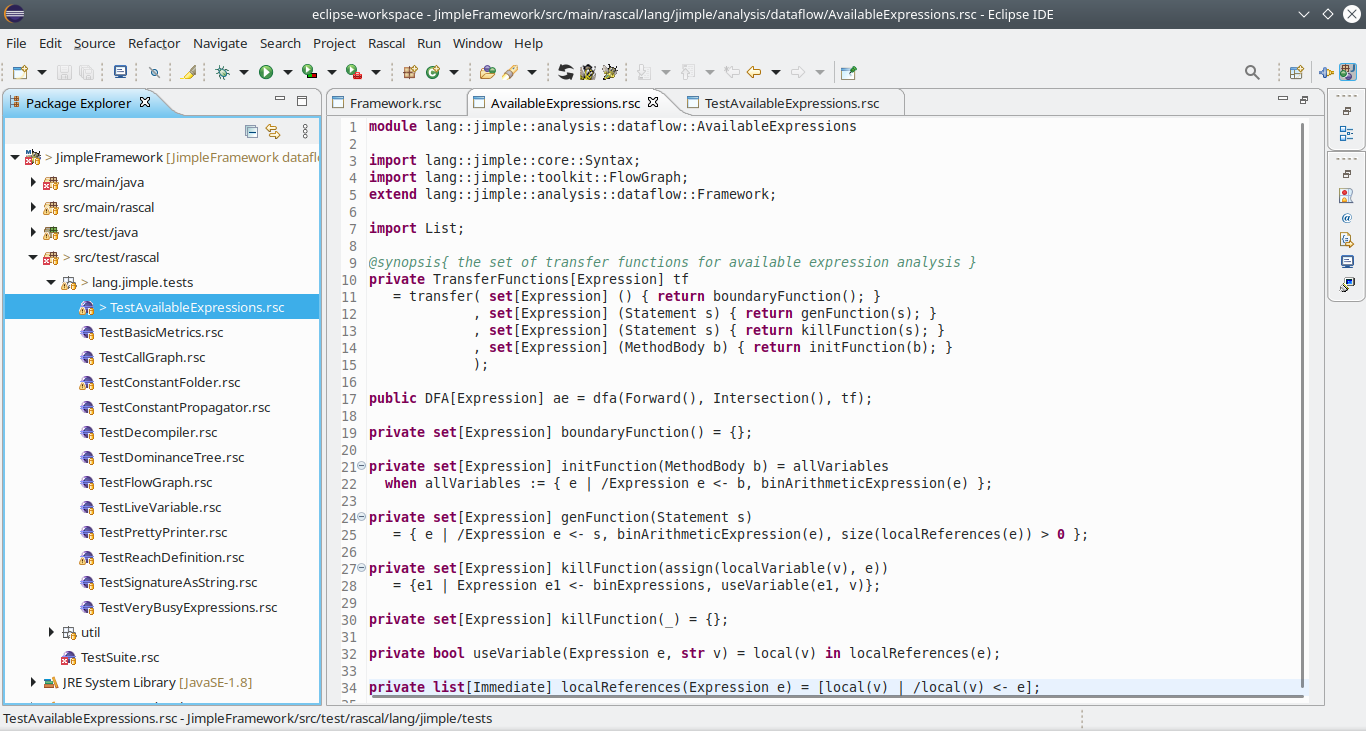
\includegraphics[width=1\textwidth]{images/jimple_framework}
	\end{center}
	\begin{center}
		\vskip -0.5cm
		\caption{\label{figure:jimple_framework}
			\small{Jimple Framework}}
		{\small{Fuente: Elaboración propia.}}
	\end{center}
\end{figure}

\begin{figure}[!ht]
	\begin{center}
		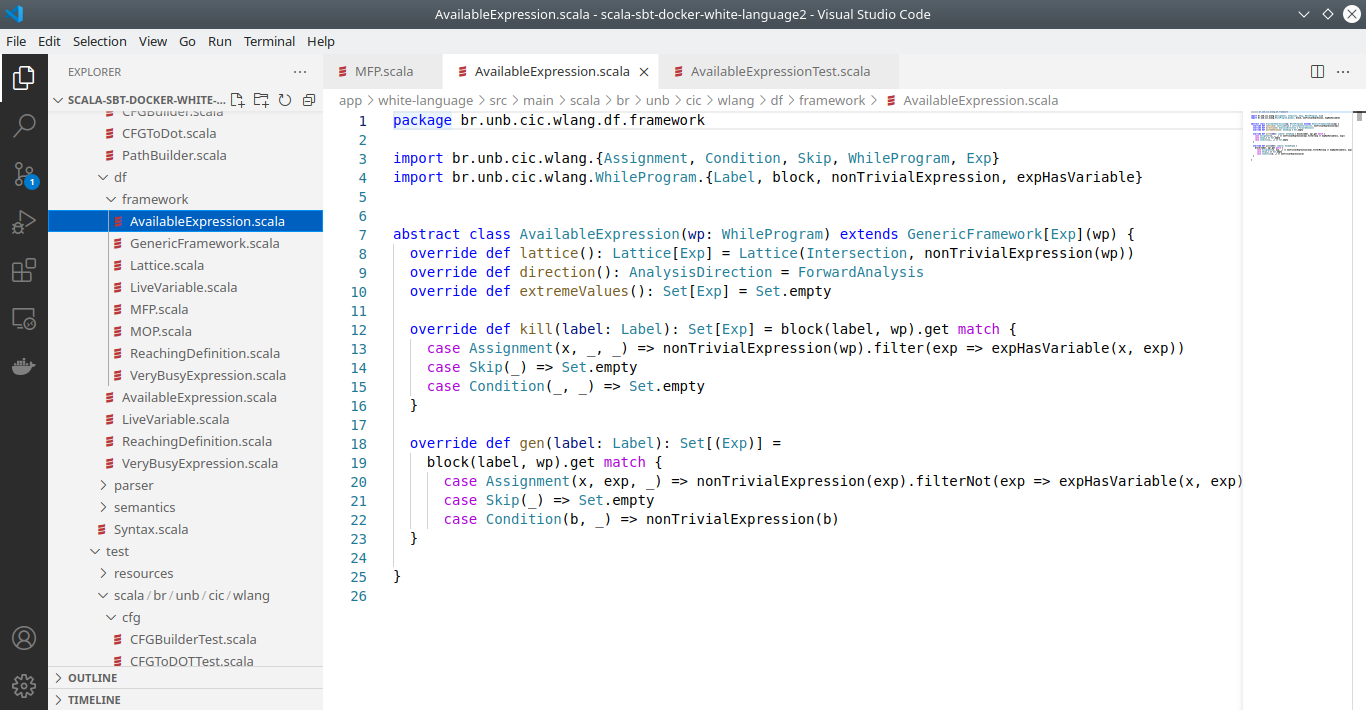
\includegraphics[width=1\textwidth]{images/while_lang}
	\end{center}
	\begin{center}
		\vskip -0.5cm
		\caption{\label{figure:while_lang}
			\small{White Language}}
		{\small{Fuente: Elaboración propia.}}
	\end{center}
\end{figure}


\subsection{Técnicas de métodos quantitativos}

As técnicas de métodos quantitativos ao usar são: comparações  pareadas, projeto ${2^3}$ e regressão linear.

\subsubsection{Comparações  Pareadas}

Nesta seção, comparamos os desempenho dos dois algoritmos (A e B). Ambos foram testados 8 vezes e seu tempo de execução é mostrado na (Figura~\ref{figure:comparacoes_pareadas_table}); alem disso, se representou numa gráfica en la (Figura~\ref{figure:comparacoes_pareadas_graph}). Os dois algoritmos usaram o mesmo padrão para obter os resultados em segundos.

\begin{figure}[!ht]
	\begin{center}
		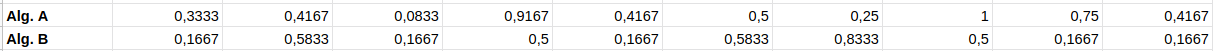
\includegraphics[width=1\textwidth]{images/comparacoes_pareadas_table}
	\end{center}
	\begin{center}
%		\vskip 0.5cm
		\caption{\label{figure:comparacoes_pareadas_table}
			\small{Comparações  Pareadas : valores}}
		{\small{Fuente: Elaboración propia.}}
	\end{center}
\end{figure}


\begin{figure}[!ht]
	\begin{center}
		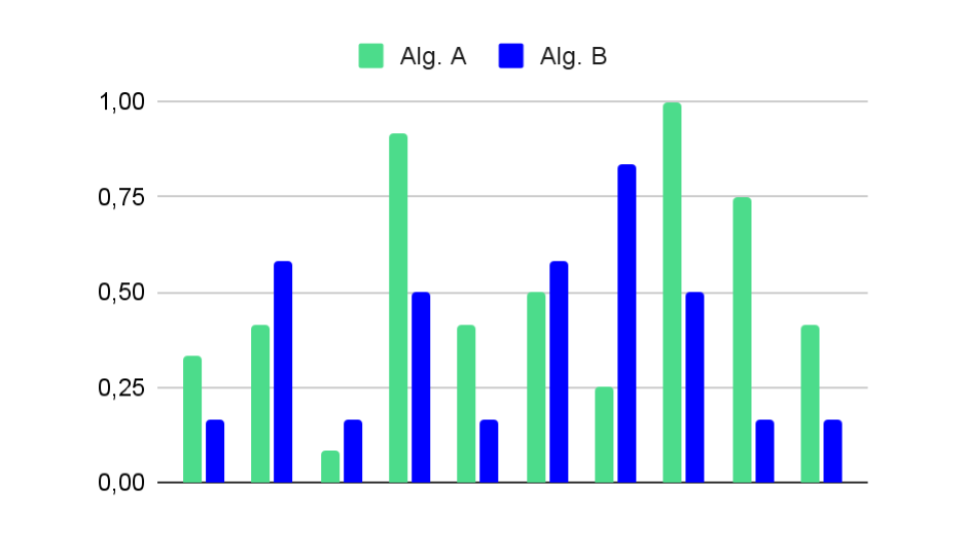
\includegraphics[width=1\textwidth]{images/comparacoes_pareadas_graph}
	\end{center}
	\begin{center}
		\vskip -0.5cm
		\caption{\label{figure:comparacoes_pareadas_graph}
			\small{Comparações  Pareadas : gráfico}}
		{\small{Fuente: Elaboración propia.}}
	\end{center}
\end{figure}

Se compararam com dois valores de intervalos.

\begin{itemize}
	\item \textbf{intervalo 90 \%}
		(-0,081 ; 0,331)

		Neste intervalo, não se pode rejeitar a hipótese já que tem o 0 entre os valores. Portanto, os algoritmos têm desempenho similar.\\
		
	\item \textbf{intervalo 80\%}
		(1,68 ; 1,99)
		
		Neste intervalo, pode-se argumentar que A tem desempenho melhor que B.\\	 
		 
\end{itemize}	

Um completo passo a passo da execução da técnica pode ser baixado aqui \attachfile{pdfs/comparacoes_pareadas_steps.pdf}

\subsubsection{Projeto ${2^3}$}

Nesta seção, analisaremos os 3 fatores que maior impacto em nosso projeto os quais são: tipo do algoritmo, tipo do sistema operativo e quantidade de processadores (Figura~\ref{figure:projeto_2_fatores}).

\begin{figure}[!ht]
	\begin{center}
		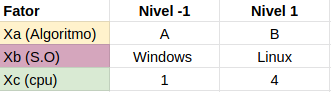
\includegraphics[width=0.5\textwidth]{images/projeto_2_fatores}
	\end{center}
	\begin{center}
		\caption{\label{figure:projeto_2_fatores}
			\small{Projeto ${2^3}$: fatores}}
		{\small{Fuente: Elaboración propia.}}
	\end{center}
\end{figure}

O projeto ${2^3}$ e seus tempos de execução em segundos são mostrado na (Figura~\ref{figure:projeto_2_valores}).

\begin{figure}[!ht]
	\begin{center}
		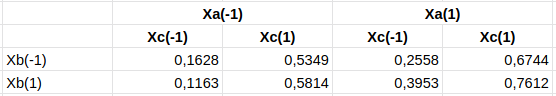
\includegraphics[width=0.7\textwidth]{images/projeto_2_valores}
	\end{center}
	\begin{center}
		\caption{\label{figure:projeto_2_valores}
			\small{Projeto ${2^3}$: valores}}
		{\small{Fuente: Elaboración propia.}}
	\end{center}
\end{figure}

A porção de variação explicada por cada fator e suas interações são mostradas na (Figura~\ref{figure:projeto_2_interacoes})

\begin{figure}[!ht]
	\begin{center}
		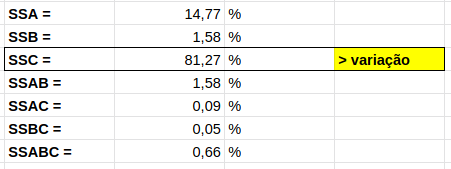
\includegraphics[width=0.7\textwidth]{images/projeto_2_interacoes}
	\end{center}
	\begin{center}
		\caption{\label{figure:projeto_2_interacoes}
			\small{Projeto ${2^3}$: interações}}
		{\small{Fuente: Elaboración propia.}}
	\end{center}
\end{figure}
	
O \textbf{``fator C''} com \textbf{81,27\%} tem a maior variação, portanto a quantidade de processadores são os que geram o maior impacto. 

Um completo passo a passo da execução da técnica pode ser baixado aqui \attachfile{pdfs/projeto_steps.pdf}

\subsubsection{Regressão Linear}

Nesta seção, examinaremos o tempo de execução em segundos do algoritmo A com quantidades diferentes de loops (for ou while) no código para poder realizar uma predição (Figura~\ref{figure:regressao_valores}).

\begin{figure}[!ht]
	\begin{center}
		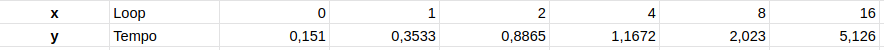
\includegraphics[width=1\textwidth]{images/regressao_valores}
	\end{center}
	\begin{center}
		\caption{\label{figure:regressao_valores}
			\small{Regressão Linear: valores}}
		{\small{Fuente: Elaboración propia.}}
	\end{center}
\end{figure}

Além disso, se apresenta um gráfico com os parâmetros de estimativa (Figura~\ref{figure:regressao_graph}) para uma melhor visualização.

\begin{figure}[!ht]
	\begin{center}
		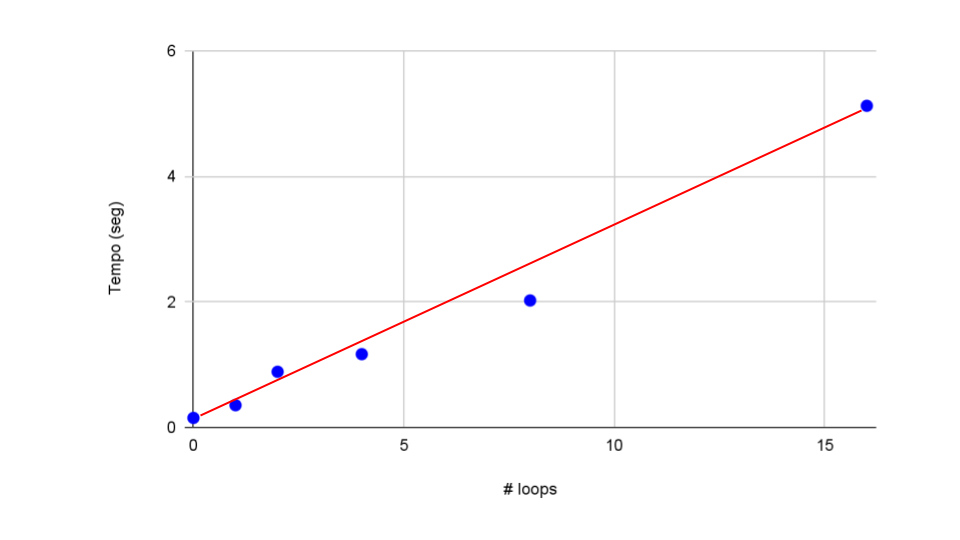
\includegraphics[width=0.9\textwidth]{images/regressao_graph}
	\end{center}
	\begin{center}
		\vskip -0.5cm
		\caption{\label{figure:regressao_graph}
			\small{Regressão Linear: gráfico}}
		{\small{Fuente: Elaboración propia.}}
	\end{center}
\end{figure}

A qualidade da regressão medida pelo coeficiente de determinação ${R^2}$ é \textbf{0,95}, portanto mostra um alto valor na regressão.

Se efetuou uma predição para um programa com 64 loops, o tempo calculado \textbf{T} é \textbf{19,27}  segundos com \textbf{90\%} o \textbf{IC} é \textbf{(18,66;19,88)}.

Um completo passo a passo da execução da técnica pode ser baixado aqui \attachfile{pdfs/regressao_steps.pdf}

\section{Conclusões}

As técnicas de métodos quantitativos colocadas em prática mostraram o seguinte:

\begin{itemize}
	\item A comparação de observações pareadas com um intervalo de 80\% revelou que o algoritmo A é melhor que o B.
	\item A execução do projeto ${2^3}$ deu como resultado que a quantidade de processadores são os que geram um maior impacto em nosso projeto. 
	\item Devido ao resultado das observações pareadas se tomou conta só do ``Algoritmo A'' com a técnica de regressão linear, a qual gerou um modelo que foi testado para um programa com 64 loops e o tempo calculado foi de 19,27 segundos.
\end{itemize}	


Como conclusão pessoal, as técnicas de métodos quantitativos são umas ferramentas interessantes no momento de comparar, analisar e até fazer uma predição. Aqueles devem ser utilizadas (ou se já estão sendo, devem ser exploradas outras técnicas) em nossos projetos.


%\bibliographystyle{sbc}
\bibliographystyle{apalike}
\bibliography{sbc-template}


\end{document}
